\begin{frame}{What is our goal?}{Motivation}
    \pause 
    \begin{block}{}<+->
        We want to \GB{efficiently} draw a \GB{uniform} random integer in an interval.
    \end{block}
    
    \onslide<+->{Where do we need this?}
    \begin{itemize}[<+->]
        \item Shuffling
        \item Graph Generators
        \item Sampling
    \end{itemize}

    \smallskip

	\begin{center}
		\onslide<.(-2)->{\includestandalone[height=3cm]{img/standalone/shuffling}}
		\hfil
		\onslide<.(-1)->{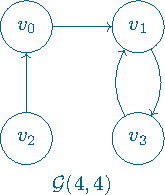
\includegraphics[height=3cm]{img/standalone/graphs}}
		\hfil
		\onslide<.->{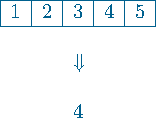
\includegraphics[height=3cm]{img/standalone/sampling}}
	\end{center}
\end{frame}